\begin{proofbox}
\textbf{\textcolor{CProof}{方法一：对数运算与普通糖水不等式（门槛最低）}}

\textbf{思路提示：} 真数同加 $c$，并不意味着对数也增加相同的数。先分别求出对数增加了多少，再比较两个分数。
\begin{description}[style=nextline, leftmargin=2.8em, labelsep=0.5em, itemsep=0.55em]
\item[\textbf{步骤1（明确原量与增加量）：}] 记 $A=\ln a,\ B=\ln b$，并记
\[P=\ln(a+c)-\ln a,\quad Q=\ln(b+c)-\ln b.\]
由于 $1<a<b$，且 $\ln x$ 严格递增，所以 $0=\ln1<A<B$。
\par\textbf{理由：} 用四个字母分别表示原来的两个高度和两个增加量，便于比较。
\item[\textbf{步骤2（分别求增加量）：}] 由 $a,b>1$，知 $a,b$ 均为正数，可以使用对数的商法则：
\begin{align*}
P&=\ln(a+c)-\ln a\\
 &=\ln\frac{a+c}{a}=\ln\left(1+\frac ca\right),\\
Q&=\ln(b+c)-\ln b\\
 &=\ln\frac{b+c}{b}=\ln\left(1+\frac cb\right).
\end{align*}
\par\textbf{理由：} $\ln u-\ln v=\ln(u/v)$，其中 $u,v>0$。
\item[\textbf{步骤3（比较两个增加量）：}] 由 $0<a<b$ 得
\[\frac1a-\frac1b=\frac{b-a}{ab}>0.\]
因此 $1/a>1/b$。乘以正数 $c$，再同加 $1$，得到
\[1+\frac ca>1+\frac cb>1.\]
两边取自然对数，得到 $P>Q>\ln1=0$。
\par\textbf{理由：} 对数函数严格递增，所以真数越大，对数值越大。
\item[\textbf{步骤4（先给分子分母同加较小增量）：}] 计算两个分数的差：
\begin{align*}
\frac{A+Q}{B+Q}-\frac AB
&=\frac{B(A+Q)-A(B+Q)}{B(B+Q)}\\
&=\frac{AB+BQ-AB-AQ}{B(B+Q)}\\
&=\frac{Q(B-A)}{B(B+Q)}>0.
\end{align*}
最后一步是因为 $Q>0, B-A>0, B>0, B+Q>0$。因此
\[\frac AB<\frac{A+Q}{B+Q}.\]
\par\textbf{理由：} 两个分数作差、通分；分子分母均为正。
\item[\textbf{步骤5（再把分子的增加量换成较大的增量）：}] 由于 $P>Q$，有 $A+P>A+Q$。分母 $B+Q>0$ 保持不变，所以
\[\frac{A+P}{B+Q}-\frac{A+Q}{B+Q}=\frac{P-Q}{B+Q}>0.\]
结合上一步，得到
\[\frac AB<\frac{A+Q}{B+Q}<\frac{A+P}{B+Q}.\]
\par\textbf{理由：} 分母相同且为正，分子越大，分数越大。
\item[\textbf{步骤6（代回原式）：}] 根据定义，
\begin{align*}
A+P&=\ln a+\ln(a+c)-\ln a=\ln(a+c),\\
B+Q&=\ln b+\ln(b+c)-\ln b=\ln(b+c).
\end{align*}
所以 $A/B<(A+P)/(B+Q)$ 就是
\[\frac{\ln a}{\ln b}<\frac{\ln(a+c)}{\ln(b+c)}.\]
\par\textbf{理由：} 将临时使用的字母还原为原式。
\item[\textbf{步骤7（证明右侧小于1）：}] 因为 $a<b$，两边加上 $c$ 得 $a+c<b+c$。又 $a+c>1$，由对数函数严格递增及 $\ln1=0$ 得
\[0<\ln(a+c)<\ln(b+c).\]
两边除以正数 $\ln(b+c)$，不等号方向不变，得到
\[0<\frac{\ln(a+c)}{\ln(b+c)}<1.\]
\par\textbf{理由：} 同加一个数不改变大小关系；除以正数不改变不等号方向。
\end{description}
\medskip
\textbf{结论回扣：} 综合左右两部分，得到
\[
\boxed{\frac{\ln a}{\ln b}<\frac{\ln(a+c)}{\ln(b+c)}<1}.
\]
\textbf{方法评价：} 无需求导；只会对数运算和分数通分就能完成。\end{proofbox}

\begin{proofbox}
\textbf{\textcolor{CProof}{方法二：直接构造函数求导（常规证明）}}

\textbf{思路提示：} 把共同增加量看成变量。原比值对应增加量为 $0$，新比值对应增加量为 $c$。只要证明比值随着增加量增大而增大，就能完成比较。
\begin{description}[style=nextline, leftmargin=2.8em, labelsep=0.5em, itemsep=0.55em]
\item[\textbf{步骤1（构造函数）：}] 固定 $a,b$，令
\[F(t)=\frac{\ln(a+t)}{\ln(b+t)},\quad t\ge0.\]
由于 $b+t>1$，分母 $\ln(b+t)>0$，函数有意义。又
\[F(0)=\frac{\ln a}{\ln b},\qquad F(c)=\frac{\ln(a+c)}{\ln(b+c)}.\]
\par\textbf{理由：} 目标是证明 $F(0)<F(c)$，而 $0<c$ 已知。
\item[\textbf{步骤2（求导并通分）：}] 令 $u(t)=\ln(a+t), v(t)=\ln(b+t)$，则
\[u'(t)=\frac1{a+t},\qquad v'(t)=\frac1{b+t}.\]
使用商的求导法则：
\begin{align*}
F'(t)&=\frac{u'v-uv'}{v^2}\\
&=\frac{\frac{\ln(b+t)}{a+t}-\frac{\ln(a+t)}{b+t}}{[\ln(b+t)]^2}\\
&=\frac{(b+t)\ln(b+t)-(a+t)\ln(a+t)}{(a+t)(b+t)[\ln(b+t)]^2}.
\end{align*}
\par\textbf{理由：} 分子两项通分，公分母为 $(a+t)(b+t)$。
\item[\textbf{步骤3（判断分母为正）：}] 由 $t\ge0$ 和 $1<a<b$，得到 $b+t>a+t>1$，因此 $a+t>0,b+t>0,\ln(b+t)>0$。所以 $(a+t)(b+t)[\ln(b+t)]^2>0$。\par\textbf{理由：} 正数的乘积仍是正数。
\item[\textbf{步骤4（判断分子为正）：}] 因为 $b+t>a+t>1$，所以 $\ln(b+t)>\ln(a+t)>0$。先固定对数因子，再固定真数因子：
\begin{align*}
(b+t)\ln(b+t)&>(a+t)\ln(b+t)\\
&>(a+t)\ln(a+t).
\end{align*}
第一步乘的是正数 $\ln(b+t)$，第二步乘的是正数 $a+t$。因此分子大于零。\par\textbf{理由：} 不等式两边乘以同一个正数，方向不变。
\item[\textbf{步骤5（应用单调性）：}] 分子与分母均为正，所以 $F'(t)>0$。函数在 $[0,+\infty)$ 连续且在 $(0,+\infty)$ 可导，故在 $[0,+\infty)$ 严格递增。由 $c>0$ 得 $F(c)>F(0)$，即
\[\frac{\ln(a+c)}{\ln(b+c)}>\frac{\ln a}{\ln b}.\]
\par\textbf{理由：} 导数恒正对应函数严格递增。
\item[\textbf{步骤6（证明右侧小于1）：}] 因为 $a<b$，两边加上 $c$ 得 $a+c<b+c$。又 $a+c>1$，由对数函数严格递增及 $\ln1=0$ 得
\[0<\ln(a+c)<\ln(b+c).\]
两边除以正数 $\ln(b+c)$，不等号方向不变，得到
\[0<\frac{\ln(a+c)}{\ln(b+c)}<1.\]
\par\textbf{理由：} 同加一个数不改变大小关系；除以正数不改变不等号方向。
\end{description}
\medskip
\textbf{结论回扣：} 综合左右两部分，得到
\[
\boxed{\frac{\ln a}{\ln b}<\frac{\ln(a+c)}{\ln(b+c)}<1}.
\]
\textbf{方法评价：} 直接研究共同增加量，适合导数与函数单调性题。\end{proofbox}

\begin{proofbox}
\textbf{\textcolor{CProof}{方法三：对数函数的凹性（几何理解）}}

\textbf{思路提示：} 对数图像向上增长，却越来越平缓。先理解图像中点的高度关系，再严格证明相同横向增量在左侧产生更大的高度增量。
\begin{description}[style=nextline, leftmargin=2.8em, labelsep=0.5em, itemsep=0.55em]
\item[\textbf{步骤1（从具体数字理解中点性质）：}] 因为 $3^2=9>8=2\times4$，由对数函数递增得 $\ln9>\ln8$，于是
\[2\ln3=\ln(3^2)>\ln(2\times4)=\ln2+\ln4.\]
两边除以正数 $2$，得到
\[\boxed{\ln3>\frac{\ln2+\ln4}{2}}.\]
图像上，横坐标 $3$ 是 $2$ 与 $4$ 的中点，曲线在这里的高度大于连接两端的线段中点高度。
\begin{center}
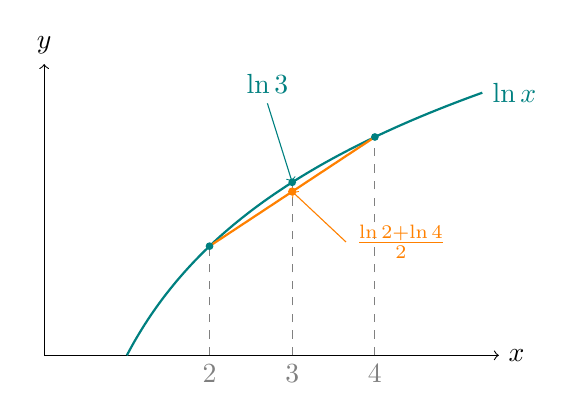
\begin{tikzpicture}[x=1.05cm,y=2cm]
\draw[->] (0,0)--(5.5,0) node[right] {$x$};
\draw[->] (0,0)--(0,1.85) node[above] {$y$};
\draw[teal,thick,domain=1:5.3,samples=100] plot (\x,{ln(\x)}) node[right] {$\ln x$};
\draw[orange,thick] (2,{ln(2)})--(4,{ln(4)});
\foreach \x in {2,3,4}{\draw[dashed,gray] (\x,0) node[below] {$\x$}--(\x,{ln(\x)});\fill[teal] (\x,{ln(\x)}) circle (1.4pt);}
\fill[orange] (3,{(ln(2)+ln(4))/2}) circle (1.5pt);
\draw[<-,teal] (3,{ln(3)})--(2.7,1.6) node[above] {$\ln3$};
\draw[<-,orange] (3,{(ln(2)+ln(4))/2})--(3.65,.72) node[right] {$\frac{\ln2+\ln4}{2}$};
\end{tikzpicture}
\end{center}\par\textbf{理由：} 对数的积与幂的运算法则。
\item[\textbf{步骤2（推广到任意两个正数）：}] 设 $u,v>0$ 且 $u\ne v$。由 $(\sqrt u-\sqrt v)^2>0$，展开得 $u+v-2\sqrt{uv}>0$，所以
\[\frac{u+v}{2}>\sqrt{uv}>0.\]
取自然对数并展开右侧：
\begin{align*}
\ln\frac{u+v}{2}&>\ln\sqrt{uv}\\
&=\ln(uv)^{1/2}\\
&=\frac12\ln(uv)=\frac{\ln u+\ln v}{2}.
\end{align*}
当 $u=v$ 时，两边相等。这就是对数函数凹性的中点形式。\par\textbf{理由：} 基本不等式与对数运算。仅凭一个数字例子不能证明一般的增加量关系，下面另作严格推导。
\item[\textbf{步骤3（证明等长区间的高度增加量递减）：}] 固定 $c>0$，令
\[G(x)=\ln(x+c)-\ln x,\quad x>0.\]
这个函数表示从横坐标 $x$ 向右移动 $c$ 后，曲线增加的高度。求导：
\begin{align*}
G'(x)&=\frac1{x+c}-\frac1x\\
&=\frac{x-(x+c)}{x(x+c)}\\
&=-\frac c{x(x+c)}<0.
\end{align*}
因为 $c>0,x>0,x+c>0$，分子为负，分母为正。故 $G(x)$ 在 $(0,+\infty)$ 严格递减。\par\textbf{理由：} 对数曲线的斜率 $1/x$ 随横坐标增大而减小，以上作差求导给出了严格的等长区间比较。
\item[\textbf{步骤4（将几何规律应用到原题）：}] 由 $a<b$ 和 $G$ 严格递减，得 $G(a)>G(b)$。又 $b+c>b$，因此 $\ln(b+c)>\ln b$，即 $G(b)>0$。合并得
\[\ln(a+c)-\ln a>\ln(b+c)-\ln b>0.\]
\begin{center}
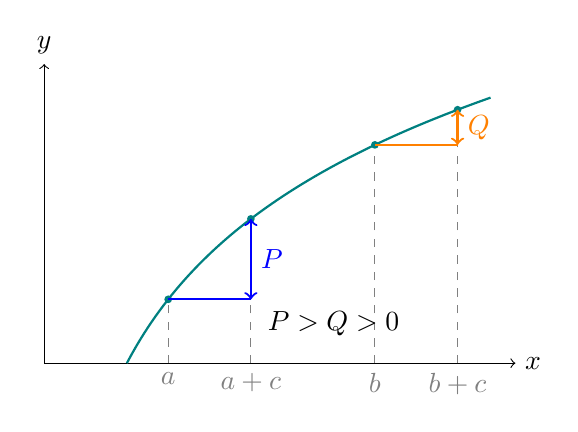
\begin{tikzpicture}[x=1.05cm,y=2cm]
\draw[->] (0,0)--(5.7,0) node[right] {$x$};
\draw[->] (0,0)--(0,1.9) node[above] {$y$};
\draw[teal,thick,domain=1:5.4,samples=100] plot (\x,{ln(\x)});
\foreach \x/\lab in {1.5/a,2.5/{a+c},4/b,5/{b+c}}{\draw[dashed,gray] (\x,0) node[below] {$\lab$}--(\x,{ln(\x)});\fill[teal] (\x,{ln(\x)}) circle (1.4pt);}
\draw[blue,thick] (1.5,{ln(1.5)})--(2.5,{ln(1.5)});
\draw[blue,<->,thick] (2.5,{ln(1.5)})--(2.5,{ln(2.5)}) node[midway,right] {$P$};
\draw[orange,thick] (4,{ln(4)})--(5,{ln(4)});
\draw[orange,<->,thick] (5,{ln(4)})--(5,{ln(5)}) node[midway,right] {$Q$};
\node at (3.5,.25) {$P>Q>0$};
\end{tikzpicture}
\end{center}图中取 $a=1.5,b=4,c=1$ 示意。即使两个横向区间重叠，前面的导数证明仍然成立。\par\textbf{理由：} 函数严格递减的定义。
\item[\textbf{步骤5（把高度关系转化为比值关系）：}] 记 $A=\ln a,\ B=\ln b$，并记
\[P=\ln(a+c)-\ln a,\quad Q=\ln(b+c)-\ln b.\]
由于 $1<a<b$，且 $\ln x$ 严格递增，所以 $0=\ln1<A<B$。
\par\textbf{理由：} 用四个字母分别表示原来的两个高度和两个增加量，便于比较。 由上一步得 $P>Q>0$。计算
\begin{align*}
\frac{A+P}{B+Q}-\frac AB
&=\frac{B(A+P)-A(B+Q)}{B(B+Q)}\\
&=\frac{AB+BP-AB-AQ}{B(B+Q)}\\
&=\frac{BP-AQ}{B(B+Q)}\\
&=\frac{B(P-Q)+Q(B-A)}{B(B+Q)}>0.
\end{align*}
因为 $B>0,P-Q>0,Q>0,B-A>0$，分子中的两项都为正；分母也为正。\par\textbf{理由：} 不能只凭图像就断定比值变大，必须完成以上分数比较。
\item[\textbf{步骤6（代回原式）：}] 由 $A+P=\ln(a+c)$、$B+Q=\ln(b+c)$、$A=\ln a$、$B=\ln b$，得到
\[\frac{\ln(a+c)}{\ln(b+c)}-\frac{\ln a}{\ln b}>0,\]
即 $\frac{\ln a}{\ln b}<\frac{\ln(a+c)}{\ln(b+c)}$。\par\textbf{理由：} 作差为正，说明前一个数大于后一个数。
\item[\textbf{步骤7（证明右侧小于1）：}] 因为 $a<b$，两边加上 $c$ 得 $a+c<b+c$。又 $a+c>1$，由对数函数严格递增及 $\ln1=0$ 得
\[0<\ln(a+c)<\ln(b+c).\]
两边除以正数 $\ln(b+c)$，不等号方向不变，得到
\[0<\frac{\ln(a+c)}{\ln(b+c)}<1.\]
\par\textbf{理由：} 同加一个数不改变大小关系；除以正数不改变不等号方向。
\end{description}
\medskip
\textbf{结论回扣：} 综合左右两部分，得到
\[
\boxed{\frac{\ln a}{\ln b}<\frac{\ln(a+c)}{\ln(b+c)}<1}.
\]
\textbf{方法评价：} 最适合理解图像本质；中点性质可用基本不等式证明，等长区间高度比较用一阶导数严格推出。\end{proofbox}

\noindent\textbf{方法四：原有辅助函数法（完整保留）}
\begin{proofbox}
	\textbf{\textcolor{CProof}{思路提示}}

	欲证原不等式左边 $\frac{\ln a}{\ln b}<\frac{\ln(a+c)}{\ln(b+c)}$，可转化为证函数 $H(x)=\frac{\ln x}{\ln(x+c)}$ 在 $(1,+\infty)$ 严格递增。右边 $\frac{\ln(a+c)}{\ln(b+c)}<1$ 由 $a+c<b+c$ 及 $\ln x$ 递增立即得到。

	\medskip
	\textbf{\textcolor{CProof}{正式推导}}
	\begin{description}[style=nextline, leftmargin=2.8em, labelsep=0.5em, itemsep=0.55em]
		\item[\textbf{步骤一（等价变形）：}] 由 $1<a<b,c>0$ 得 $\ln a,\ln b,\ln(a+c),\ln(b+c)$ 均为正数。原不等式左边两边同乘正数 $\ln b\cdot\ln(b+c)$，得到：
			\[
				\ln a\cdot\ln(b+c)<\ln b\cdot\ln(a+c).
			\]
			再将两边同除以正数 $\ln(a+c)\cdot\ln(b+c)$，得到
			\[
				\frac{\ln a}{\ln(a+c)}<\frac{\ln b}{\ln(b+c)}.
			\]
			故定义函数 $H(x)=\dfrac{\ln x}{\ln(x+c)},\quad x>1$。
			\par\textbf{理由：} 由 $a,b>1$ 及 $c>0$ 知 $\ln(a+c),\ln(b+c)>0$，交叉相乘不等号方向不变。

		\item[\textbf{步骤二（求导）：}] 固定 $c$，设 $u(x)=\ln x$、$v(x)=\ln(x+c)$，则 $u'(x)=1/x$、$v'(x)=1/(x+c)$。代入商的求导法则，得到：
			\[
				H'(x)=\frac{\frac{1}{x}\ln(x+c)-\ln x\cdot\frac{1}{x+c}}{[\ln(x+c)]^{2}}.
			\]
			\par\textbf{理由：} 商数求导法则 $(u/v)'=(u'v-uv')/v^{2}$。

		\item[\textbf{步骤三（判号）：}] 考虑分子：
			\[
				M(x)=\frac{\ln(x+c)}{x}-\frac{\ln x}{x+c}.
			\]
			通分得到
\[
M(x)=\frac{(x+c)\ln(x+c)-x\ln x}{x(x+c)}.
\]
由于 $x>1,c>0$，分母 $x(x+c)>0$，所以只需判断分子是否大于零。由于 $x+c>x>1$，考察函数 $\psi(t)=t\ln t$。由乘积求导法则，$\psi'(t)=1\cdot\ln t+t\cdot(1/t)=\ln t+1$。因为 $t>1$，所以 $\ln t>0$，从而 $\psi'(t)>0$，故 $\psi(t)$ 严格递增。由 $x+c>x$ 得
			\[
				(x+c)\ln(x+c)>x\ln x.
			\]
			两边除以 $x(x+c)$ 得
			\[
				\frac{\ln(x+c)}{x}>\frac{\ln x}{x+c}.
			\]
			因此 $M(x)>0$。又 $x+c>1$，所以 $\ln(x+c)>0$，其平方也为正。由 $H'(x)=M(x)/[\ln(x+c)]^2$ 得 $H'(x)>0$。
			\par\textbf{理由：} 分子正负决定导数符号，利用 $\psi(t)$ 单调性比较。

		\item[\textbf{步骤四（单调性应用）：}] $H'(x)>0$ 说明 $H(x)$ 在 $(1,+\infty)$ 严格递增。因为 $a<b$，所以 $H(a)<H(b)$，即
			\[
				\frac{\ln a}{\ln(a+c)}<\frac{\ln b}{\ln(b+c)}.
			\]
			两边同乘正数 $\ln(a+c)\ln(b+c)$ 得
\[\ln a\ln(b+c)<\ln b\ln(a+c).\]
再同除以正数 $\ln b\ln(b+c)$，得到
			\[
				\frac{\ln a}{\ln b}<\frac{\ln(a+c)}{\ln(b+c)}.
			\]
			\par\textbf{理由：} 单调递增定义与交叉乘的可逆性。

		\item[\textbf{步骤五（右边不等式）：}] 由 $a<b$ 及 $c>0$ 得 $a+c<b+c$。又 $\ln x$ 在 $(0,+\infty)$ 递增，故 $\ln(a+c)<\ln(b+c)$。又 $b+c>1$，所以 $\ln(b+c)>0$。两边除以该正数，得到
\[
\frac{\ln(a+c)}{\ln(b+c)}<1.
			\]
			\par\textbf{理由：} 对数函数单调性。
	\end{description}

	\medskip
	\textbf{\textcolor{CProof}{结论回扣}}

	综合左右两部分，原不等式链 $\dfrac{\ln a}{\ln b}<\dfrac{\ln(a+c)}{\ln(b+c)}<1$ 得证。左边依靠构造函数 $H(x)$ 单调性，右边直接利用真数大小。
\end{proofbox}

\noindent\textbf{方法五：做差凑项与增长量放缩法（无需导数）}
\begin{proofbox}
\textbf{\textcolor{CProof}{思路提示}}

先做差，再寻找差式的下界。直接比较两个对数的高度遇到困难时，改为比较它们各自增加的高度。这一思路来自对数函数越往右增长越慢的特点。

\begin{description}[style=nextline, leftmargin=2.8em, labelsep=0.5em, itemsep=0.55em]
\item[\textbf{步骤1（做差、通分）：}] 因为 $1<a<b$ 且 $c>0$，所以 $\ln b>0$，$\ln(b+c)>0$。设
\begin{align*}
D&=\frac{\ln(a+c)}{\ln(b+c)}-\frac{\ln a}{\ln b}\\
&=\frac{\ln(a+c)\ln b}{\ln b\ln(b+c)}-\frac{\ln a\ln(b+c)}{\ln b\ln(b+c)}\\
&=\frac{\ln(a+c)\ln b-\ln(b+c)\ln a}{\ln b\ln(b+c)}.
\end{align*}
记分子为 $N=\ln(a+c)\ln b-\ln(b+c)\ln a$。由于分母为正，只要证明 $N>0$，就能证明 $D>0$。
\par\textbf{理由：} 通分不改变分数的值；分母为正时，分数与分子同号。

\item[\textbf{步骤2（为什么直接利用中点性质放缩会卡住）：}] 由基本不等式，$\dfrac{a+c}{2}\geq\sqrt{ac}$，两边取自然对数，再加 $\ln2$，得到
\begin{align*}
\ln(a+c)&=\ln\frac{a+c}{2}+\ln2\\
&\geq\ln\sqrt{ac}+\ln2\\
&=\frac{\ln a+\ln c}{2}+\ln2.
\end{align*}
同理，$\ln(b+c)\geq\dfrac{\ln b+\ln c}{2}+\ln2$。两式分别在 $a=c$、$b=c$ 时取等号。

由于 $\ln b>0$，第一式乘以 $\ln b$ 后给出正项的下界；但由于 $-\ln a<0$，第二式乘以 $-\ln a$ 后不等号反向，得到的是负项的上界。一个下界与一个上界相加，不能确定原差式的下界。故不能将两个下界直接代入 $N$ 后断定 $N>0$。
\par\textbf{理由：} 要证明差为正，应放小被减数或放大减数；不能把被减数与减数同时放小后就判断原差的正负。

\item[\textbf{步骤3（从高度转向增长量）：}] 例如 $3^2=9>8=2\cdot4$，取自然对数得到 $2\ln3>\ln2+\ln4$。移项得到
\[\ln3-\ln2>\ln4-\ln3.\]
这说明横坐标同样增加 $1$，从 $2$ 到 $3$ 的高度增加量大于从 $3$ 到 $4$ 的高度增加量。于是尝试比较
\[P=\ln(a+c)-\ln a,\qquad Q=\ln(b+c)-\ln b.\]
\par\textbf{理由：} 对数图像越往右增长越慢；具体例子启发我们比较一般的增长量，但例子本身不能代替一般证明。

\item[\textbf{步骤4（严格比较增长量，无需求导）：}]
\begin{align*}
P&=\ln\frac{a+c}{a}=\ln\left(1+\frac ca\right),\\
Q&=\ln\frac{b+c}{b}=\ln\left(1+\frac cb\right).
\end{align*}
因为 $a,b,c>0$ 且 $b>a$，所以
\[\frac ca-\frac cb=\frac{c(b-a)}{ab}>0.\]
因此 $1+c/a>1+c/b>1$。由自然对数严格递增，得到
\[P>Q>\ln1=0.\]
\par\textbf{理由：} 对数的商法则、正数乘除的符号规则和对数函数的单调性。

\item[\textbf{步骤5（凑项、分组）：}] 为了在原分子中构造 $P$ 与 $Q$，加上再减去同一个数 $\ln a\ln b$：
\begin{align*}
N&=\ln(a+c)\ln b-\ln a\ln b\\
 &\quad+\ln a\ln b-\ln(b+c)\ln a\\
&=[\ln(a+c)-\ln a]\ln b\\
&\quad-[\ln(b+c)-\ln b]\ln a\\
&=P\ln b-Q\ln a.
\end{align*}
\par\textbf{理由：} 加减同一个数不改变原式；分组后提取公因式。

\item[\textbf{步骤6（只放小正项）：}] 因为 $P>Q$ 且 $\ln b>0$，所以 $P\ln b>Q\ln b$。两边同时减去 $Q\ln a$，得到
\begin{align*}
N&=P\ln b-Q\ln a\\
&>Q\ln b-Q\ln a\\
&=Q(\ln b-\ln a).
\end{align*}
又因为 $Q>0$，且 $b>a>1$，所以 $\ln b-\ln a>0$。两个正数相乘为正，故 $N>0$。
\par\textbf{理由：} 只放小正项，保持被减项不变，得到原差式的严格下界。

\item[\textbf{步骤7（回到原不等式）：}] 由步骤1，$D=N/[\ln b\ln(b+c)]>0$，因此
\[\frac{\ln a}{\ln b}<\frac{\ln(a+c)}{\ln(b+c)}.\]
又 $1<a+c<b+c$，取自然对数得 $0<\ln(a+c)<\ln(b+c)$。两边除以正数 $\ln(b+c)$，得到 $\ln(a+c)/\ln(b+c)<1$。
\end{description}
\medskip
\textbf{\textcolor{CProof}{结论回扣}}
\[\boxed{\frac{\ln a}{\ln b}<\frac{\ln(a+c)}{\ln(b+c)}<1}.\]
\textbf{方法评价：} 与方法一共享增长量比较的基础，与方法三共享凹性的直观思想，但本方法专门展示做差遇到放缩障碍后如何凑项、改变比较对象并只放小正项。无需导数。记住：直接比较高度不方便时，可以尝试比较增长量。
\end{proofbox}
